\documentclass[12pt,a4paper, twoside, notitlepage]{report}

\usepackage{geometry}

\usepackage[utf8]{inputenc}
\usepackage[english,greek]{babel}
\usepackage{alphabeta} 

\usepackage{titling} %Add title page
\usepackage{abstract} %Add abstract
\usepackage{ragged2e} %Modify Abstract

\usepackage{fancyhdr} %Add header and footer

\usepackage{tocloft} %add table of contents
\usepackage{titletoc} %modify titles in toc
\usepackage{setspace} %modify space in toc

\usepackage{appendix}
\usepackage{titlesec} %modify appendix

\usepackage[bookmarks == true]{hyperref} %pdf bookmarks
\usepackage[open, openlevel = 0]{bookmark} %pdf bookmarks

\usepackage{listings} %code block
\usepackage{xcolor} %colors for code block

\usepackage{tcolorbox}

\usepackage{natbib} %for bibliotek
\usepackage{cite}

\usepackage{enumitem} %Bullets Points
\usepackage{pifont} %Bullets Points Style

\usepackage{graphicx} %Insert Images
\usepackage{caption} %Insert Caption Images

\usepackage{float}
\usepackage{hyphenat}

\usepackage{amssymb}

%---------------------------------------------------------------------------------------------------------------
\geometry{left=1in, right=1in, top=1in, bottom=1in}

\setlength{\headheight}{14.5pt}  %solution for warnings
\addtolength{\topmargin}{-2.5pt}  %solution for warnings

%---------------------------------------------------------------------------------------------------------------
\fancypagestyle{mystyle}{
    \fancyhf{}
    \fancyhead[R]{\foreignlanguage{greek}{Βάσεις Δεδομένων}}
    \renewcommand{\footrulewidth}{0.4pt}% default is 0pt
    \fancyfoot[L]{\foreignlanguage{greek}{Ομάδα: 8}}
    \fancyfoot[C]{\thepage}
    \fancyfoot[R]{2023-2024}
}

%---------------------------------------------------------------------------------------------------------------
\renewenvironment{abstract}{\normalsize\quotation\centering\textbf{\Large\abstractname}\vspace{1em}\par\justifying}

%---------------------------------------------------------------------------------------------------------------
\titlecontents{chapter}[0em]{\bfseries\Large}{}{}{\titlerule*[1pc]{.}\contentspage}
\titlecontents{section}[1em]{\normalfont\large}{\thecontentslabel\quad}{}{\titlerule*[1pc]{.}\contentspage}
\titlecontents{subsection}[2em]{\normalfont}{\thecontentslabel\quad}{}{\titlerule*[1pc]{.}\contentspage}

%---------------------------------------------------------------------------------------------------------------
\definecolor{vscode-light-bg}{RGB}{240,240,240}   % Light gray background
\definecolor{vscode-dark-fg}{RGB}{34,34,34}        % Dark foreground
\definecolor{vscode-dark-comment}{RGB}{128,128,128} % Dark gray comments
\definecolor{vscode-dark-string}{RGB}{255,125,0}   % Orange strings
\definecolor{vscode-dark-keyword}{RGB}{170,43,226}  % Dark purple keywords

\lstset{
  language=SQL,
  basicstyle=\color{vscode-dark-fg}\small\ttfamily,
  keywordstyle=\color{vscode-dark-keyword},
  commentstyle=\color{vscode-dark-comment},
  stringstyle=\color{vscode-dark-string},
  showstringspaces=false,
  frame=single,
  rulecolor=\color{gray!50},     % Set the color of the frame
  backgroundcolor=\color{gray!2},
  numbers=left,               % Add line numbers to the left
  numberstyle=\small\color{gray},  % Styling for line numbers
  stepnumber=1,               % Line numbers every step line
  numbersep=10pt,               % Space between line numbers and code
  numberstyle=\small\color{black!70},  % Bigger and darker line numbers
}

%---------------------------------------------------------------------------------------------------------------
\begin{document}

\pagestyle{mystyle}

%---------------------------------------------------------------------------------------------------------------
\phantomsection
\bookmark[page=1, level=0]{Εξώφυλλο}
\thispagestyle{empty}
\begin{titlepage} 
    \thispagestyle{empty}
    \center
    \large{Δημοκρίτειο Πανεπιστήμιο Θράκης} \\ [0.2cm]
    \large {Τμήμα Ηλεκτρολόγων Μηχανικών και Μηχανικών Υπολογιστών} \\ [1.5cm]

    \begin{tabular}[t]{@{}l} 
      Ομάδα: 8
    \end{tabular}
    \hfill% move it to the right
    \begin{tabular}[t]{l@{}}
       Ιανουάριος 10, 2024
    \end{tabular}

    \vspace{2.0cm}
    \huge {\bfseries {Βάσεις Δεδομένων - Εργασία}} \\[0.2cm]
    \Large {\bfseries {\selectlanguage{english}{Database Driven Website - Moving On}}} \\[0.5cm]

    \selectlanguage{greek}
    \vspace{0.6cm}
    \begin{tabular}{ll}
        \large{Βασιλική Ειρήνη Μηλιούδη Σίσκου}    &  \large{ΧΧΧΧΧ} \\
        \large{Θανάσης Τσιρίκας}  &  \large{ΧΧΧΧΧ} \\
        \large{Παναγιώτα Νεφέλη Κουλιούμπα}     &  \large{ΧΧΧΧΧ} \\
    \end{tabular}

    \vspace{1.0cm}
    \begin{abstract}
        \noindent O σχεδιασμός της βάσης δεδομένων εστιάζει στην αποθήκευση πληροφοριών για μια μικρή μεταφορική εταιρεία. Μετά από ανάλυση απαιτήσεων, δημιουργήθηκαν τα διαγράμματα οντοτήτων–συσχετίσεων(Ο-Σ) και το σχεσιακό, τα οποία αποτέλεσαν τη βάση για την ανάπτυξη του κώδικα. Η εφαρμογή των παραπάνω θα έχει ως αποτέλεσμα τη δημιουργία ιστοσελίδας, η οποία θα ενσωματώνει μέρος της παραπάνω βάσης δεδομένων.
    \end{abstract}
\end{titlepage}

\phantomsection
\bookmark[page=2,level=0]{Περιεχόμενα}
\singlespacing
\tableofcontents
\singlespacing
\newpage

\pagenumbering{arabic}
\renewcommand{\chaptername}{Μέρος}
\chapter[Μέρος 1: Σχεδιασμός Βάσης Δεδομένων]{Σχεδιασμός Βάσης Δεδομένων}
Ο κάθε \textit{γραμματέας} \textbf{διαχειρίζεται} (\foreignlanguage{english}{\textbf{manages}}) \textit{οδηγούς} και \textbf{καταγράφει/επεξεργάζεται} (\foreignlanguage{english}{\textbf{records}}) \textit{παραγγελίες}. 
Κάθε \textit{πελάτης} \textbf{καταχωρεί} (\foreignlanguage{english}{\textbf{places}}) τουλάχιστον μία \textit{παραγγελία} και \textbf{πραγματοποιεί} (\foreignlanguage{english}{\textbf{makes}}) την αντίστοιχη \textit{πληρωμή}.
Η \textit{παραγγελία} \textbf{έχει} (\foreignlanguage{english}{\textbf{has}}) την αντίστοιχη \textit{πληρωμή} και μπορεί να \textbf{περάσει} (\foreignlanguage{english}{\textbf{is going into}}) στο στάδιο της \textit{παράδοσης}. 
Ένας \textit{οδηγός} μπορεί να \textbf{παραδώσει} (\foreignlanguage{english}{\textbf{carries out}}) την \textit{παραγγελία}. 
Ένα \textit{φορτηγό} μπορεί να \textbf{μεταφέρει} (\foreignlanguage{english}{\textbf{transfers}}) μια \textit{παράδοση}. \\

\noindent Οι βασικές οντότητες που θα περιλαμβάνονται στη βάση δεδομένων  είναι: \\ [0.3cm]
Για κάθε γραμματέα (\foreignlanguage{english}{SECRETARY}) θα αποθηκεύονται:

%------------------------------------------------------------------------------------------
\vspace{-0.2em} 
\begin{itemize}[itemsep=-0.1em]
    \item[\ding{213}] \textit{αριθμός ταυτότητας} (\foreignlanguage{english}{\textit{ID}})
    \item[\ding{213}] \textit{όνομα} (\foreignlanguage{english}{\textit{first name}})
    \item[\ding{213}] \textit{επίθετο} (\foreignlanguage{english}{\textit{last name}})
    \item[\ding{213}] \textit{τηλέφωνο }(\foreignlanguage{english}{\textit{phone}}) 
    \item[\ding{213}] \textit{όνομα χρήστη} (\foreignlanguage{english}{\textit{username}})
    \item[\ding{213}] \textit{κωδικός πρόσβασης} (\foreignlanguage{english}{\textit{password}})
\end{itemize}
\vspace{-0.1em} 
\textbf{Πρωτεύον Κλειδί: \foreignlanguage{english}{\underline{ID}}}
\vspace{0.5em} 

%------------------------------------------------------------------------------------------
\noindent Για κάθε οδηγό (\foreignlanguage{english}{DRIVER}) θα αποθηκεύονται:
\vspace{-0.4em} 
\begin{itemize}[itemsep=-0.2em]
    \item[\ding{213}] \textit{αριθμός ταυτότητας} (\foreignlanguage{english}{\textit{ID}})
    \item[\ding{213}] \textit{όνομα} (\foreignlanguage{english}{\textit{first name}})
    \item[\ding{213}] \textit{επίθετο} (\foreignlanguage{english}{\textit{last name}}) 
    \item[\ding{213}] \textit{τηλέφωνο} (\foreignlanguage{english}{\textit{phone}})
\end{itemize}
\vspace{-0.1em} 
\textbf{Πρωτεύον Κλειδί: \foreignlanguage{english}{\underline{ID}}}
\vspace{0.5em} 

%---------------------------------------------------------------------------------------
\noindent Για κάθε όχημα (\foreignlanguage{english}{TRUCK}) θα αποθηκεύονται: 
\vspace{-0.4em} 
\begin{itemize}[itemsep=-0.2em]
    \item[\ding{213}] \textit{αριθμός πινακίδας} (\foreignlanguage{english}{\textit{ID}})
    \item[\ding{213}] \textit{έτος αγοράς} (\foreignlanguage{english}{\textit{purchase year}}) 
    \item[\ding{213}] \textit{έτος παραγωγής} (\foreignlanguage{english}{\textit{production year}})
    \item[\ding{213}] \textit{χωρητικότητα} (\foreignlanguage{english}{\textit{capacity}})
    \item[\ding{213}] \textit{εταιρεία παραγωγής }(\foreignlanguage{english}{\textit{manufacturer}})
\end{itemize}
\vspace{-0.1em} 
\textbf{Πρωτεύον Κλειδί: \foreignlanguage{english}{\underline{ID}}}
\vspace{0.5em} 

%---------------------------------------------------------------------------------------
\noindent Για κάθε πελάτη (\foreignlanguage{english}{CLIENT}) θα αποθηκεύονται: 
\vspace{-0.4em} 
\begin{itemize}[itemsep=-0.2em]
    \item[\ding{213}] \textit{αριθμός ταυτότητας} (\foreignlanguage{english}{\textit{ID}})
    \item[\ding{213}] \textit{όνομα} (\foreignlanguage{english}{\textit{first name}})
    \item[\ding{213}] \textit{επίθετο} (\foreignlanguage{english}{\textit{last name}})
    \item[\ding{213}] \textit{τηλέφωνο} (\foreignlanguage{english}{\textit{phone}}) 
\end{itemize}
\vspace{-0.1em} 
\textbf{Πρωτεύον Κλειδί: \foreignlanguage{english}{\underline{ID}}}
\vspace{0.5em} 

%---------------------------------------------------------------------------------------
\noindent Για καθε πληρωμή (\foreignlanguage{english}{PAYMENT}) θα αποθηκεύονται: 
\vspace{-0.4em} 
\begin{itemize}[itemsep=-0.2em]
    \item[\ding{213}] \textit{αριθμός πληρωμής} (\foreignlanguage{english}{\textit{ID}})
    \item[\ding{213}] \textit{ημερομηνία} (\foreignlanguage{english}{\textit{date}})
    \item[\ding{213}] \textit{μέθοδος πληρωμής} (\foreignlanguage{english}{\textit{method}})
    \item[\ding{213}] \textit{ποσό πληρωμής} (\foreignlanguage{english}{\textit{amount}})
\end{itemize}
\vspace{-0.1em} 
\textbf{Πρωτεύον Κλειδί: \foreignlanguage{english}{\underline{ID}}} 
\hfill \break
\textbf{Ξένο Κλειδί: \foreignlanguage{english}{\underline{orderID}, \underline{clientID}}}
\vspace{0.5em} 

%---------------------------------------------------------------------------------------
\noindent Για κάθε παραγγελία (\foreignlanguage{english}{ORDER}) θα αποθηκεύονται: 
\vspace{-0.4em} 
\begin{itemize}[itemsep=-0.2em]
    \item[\ding{213}] \textit{αριθμός παραγγελίας} (\foreignlanguage{english}{\textit{ID}})
    \item[\ding{213}] \textit{τιμή} (\foreignlanguage{english}{\textit{price}})
    \item[\ding{213}] \textit{κατάσταση} (\foreignlanguage{english}{\textit{status}})
\end{itemize}
\vspace{-0.1em} 
\textbf{Πρωτεύον Κλειδί: \foreignlanguage{english}{\underline{ID}}}
\vspace{0.5em} 

%---------------------------------------------------------------------------------------
\noindent Για κάθε παράδοση (\foreignlanguage{english}{DELIVERY}) θα αποθηκεύονται:
\vspace{-0.4em} 
\begin{itemize}
    \item[\ding{213}] \textit{αριθμός παράδοσης} (\foreignlanguage{english}{\textit{ID}})
    \item[\ding{213}] \textit{ημερομηνία παράδοσης} (\foreignlanguage{english}{\textit{date}})
    \item[\ding{213}] \textit{πληροφορίες παραλαβής} (\foreignlanguage{english}{\textit{pick up}}) και \textit{παράδοσης} (\foreignlanguage{english}{\textit{delivery}})
    \item[\ding{213}] Τόσο η παράδοση (\foreignlanguage{english}{delivery}) όσο και η παραλαβή (\foreignlanguage{english}{pick up}) αποτελούνται από:
        \begin{itemize}[itemsep=0.2em]
            \item[\ding{213}] \textit{ταχυδρομικό κώδικα} (\foreignlanguage{english}{\textit{postal code}})
            \item[\ding{213}] \textit{πόλη} (\foreignlanguage{english}{\textit{city}})
            \item[\ding{213}] \textit{οδό} (\foreignlanguage{english}{\textit{street}})
            \item[\ding{213}]  \textit{αριθμό} (\foreignlanguage{english}{\textit{number}})
 \end{itemize} 
\end{itemize}
\vspace{-0.1em} 
\quad\textbf{Πρωτεύον Κλειδί: \foreignlanguage{english}{\underline{orderID}, \underline{ID}}} \\ [0.3cm]
%---------------------------------------------------------------------------------------
\indent Η οντότητα \foreignlanguage{english}{DELIVERY} εξρτάται(μη ισχυρή οντότητα) από την οντότητα \foreignlanguage{english}{ORDER} καθώς δεν υφίστανται χωρίς να έχει προηγηθεί η ύπαρξη μιας παραγγελίας.
Η ιδιότητα \foreignlanguage{english}{phone} του \foreignlanguage{english}{CLIENT} είναι πλειότιμο, δηλαδή ένας πελάτης μπορεί να έχει παραπάνω από ένα τηλέφωνο.
Τέλος, η ιδιότητα \foreignlanguage{english}{amount} της \foreignlanguage{english}{PAYMENT} είναι παραγόμενο μέγεθος της ιδιότητας  \foreignlanguage{english}{price} της \foreignlanguage{english}{ORDER}.


\begin{figure}
  \centering
      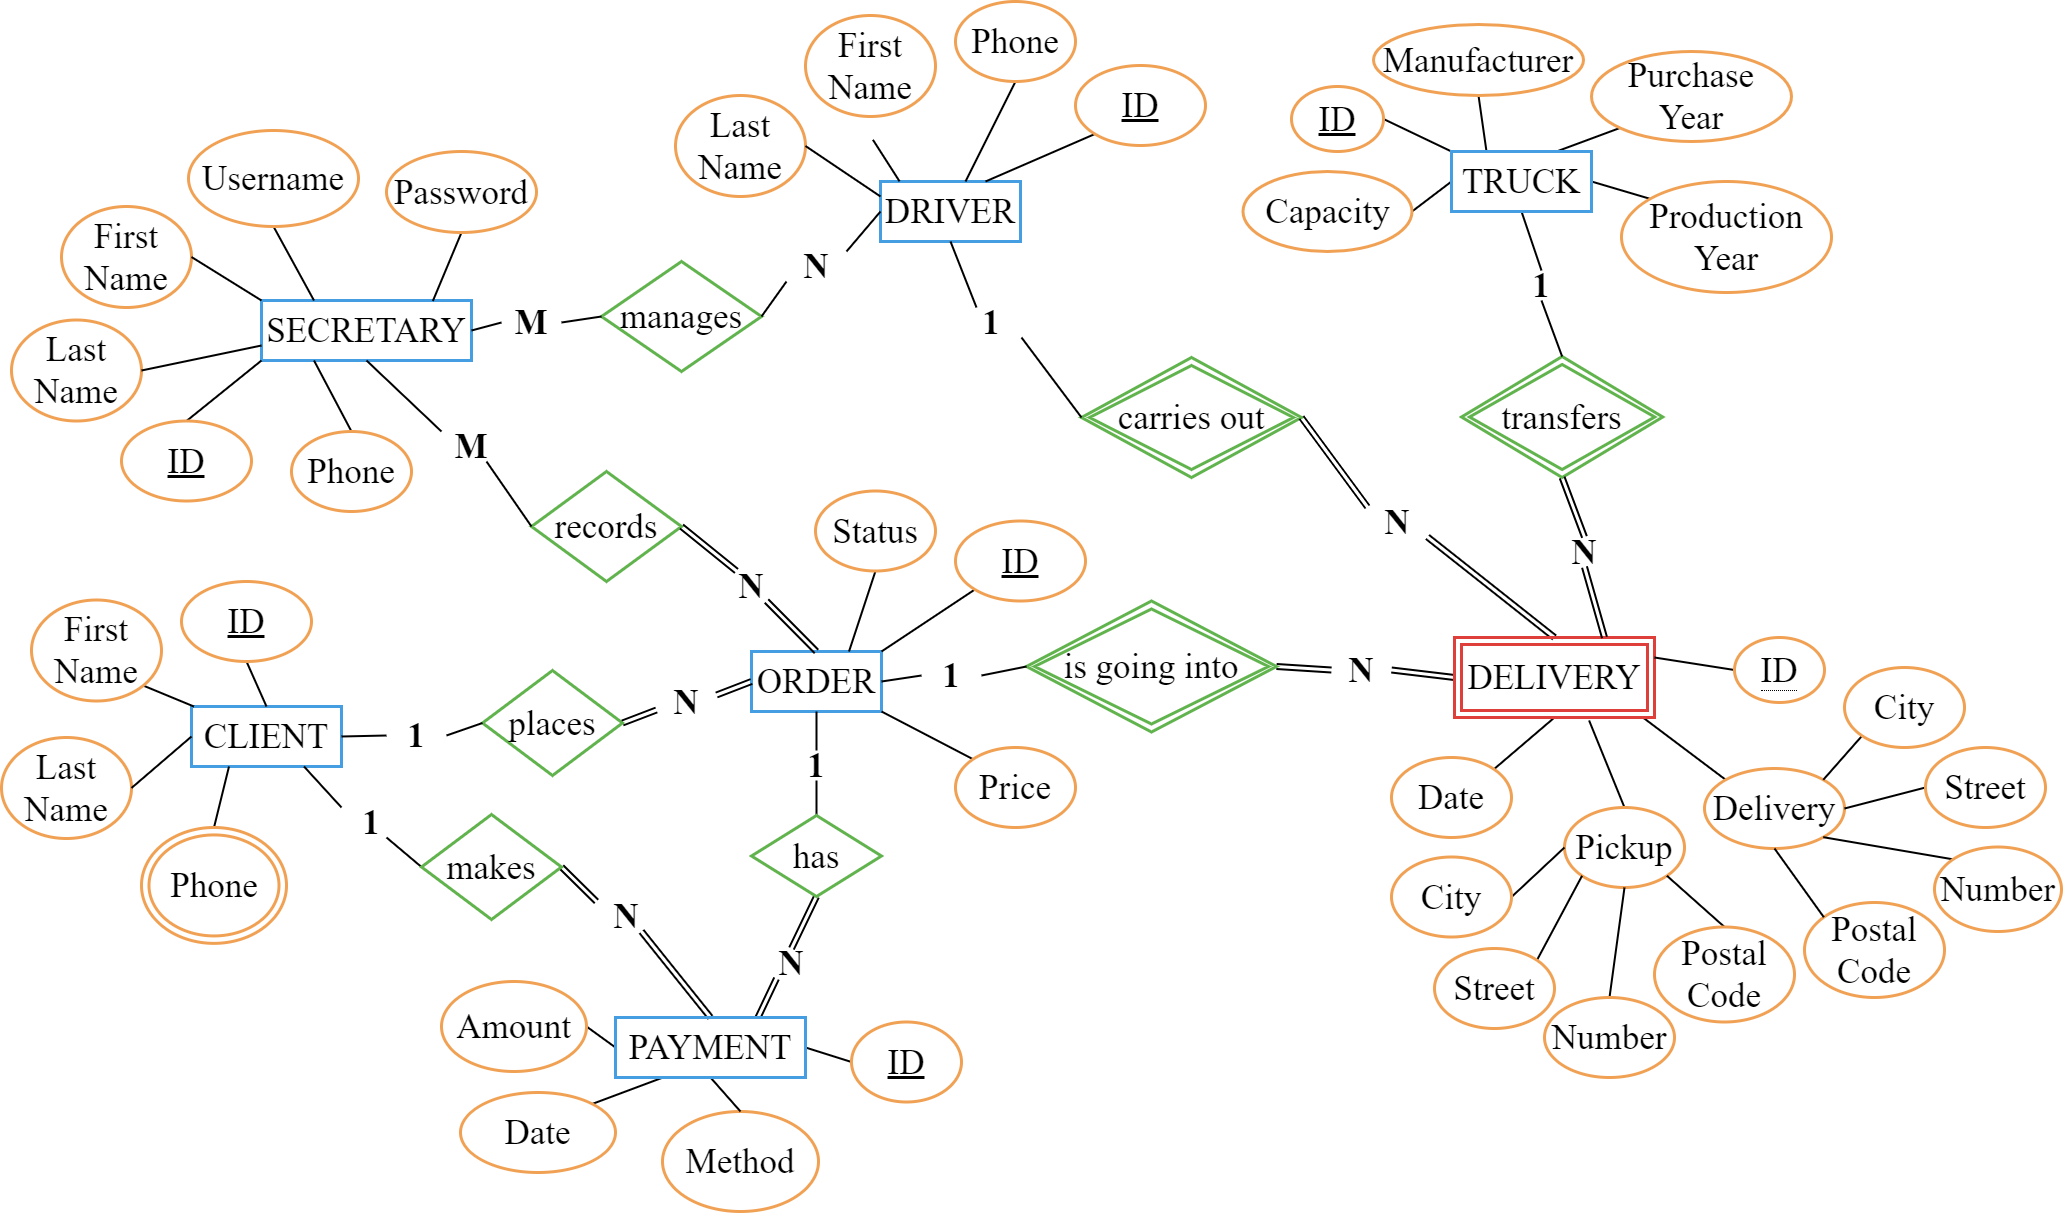
\includegraphics[width=1\textwidth]{images/ER.png}
  \captionsetup{labelfont=bf}
  \caption{Διάγραμμα Οντοτήτων - Συσχετίσεων}
\end{figure}

\phantomsection
\addcontentsline{toc}{section}{\protect\numberline{1.1}Διάγραμμα Οντοτήτων - Συσχετίσεων}

\newpage
\renewcommand{\chaptername}{Μέρος}
\chapter[Μέρος 2: Ανάπτυξη Βάσης Δεδομένων]{Ανάπτυξη Βάσης Δεδομένων}
\noindentΟι πληροφορίες που δεν απεικονίζονται στο διάγραμμα είναι οι εξής: \\
Η ιδιότητα \foreignlanguage{english}{status} μπορεί να πάρει τις τιμές '\foreignlanguage{english}{Received}', '\foreignlanguage{english}{Cancel}', '\foreignlanguage{english}{Done}' και η ιδιότητα \foreignlanguage{english}{method} μπορεί να πάρει τις τιμές '\foreignlanguage{english}{Card}' και '\foreignlanguage{english}{Cash}'.

\section{Σχεσιακό Διάγραμμα}
\begin{figure}[h]
  \centering
      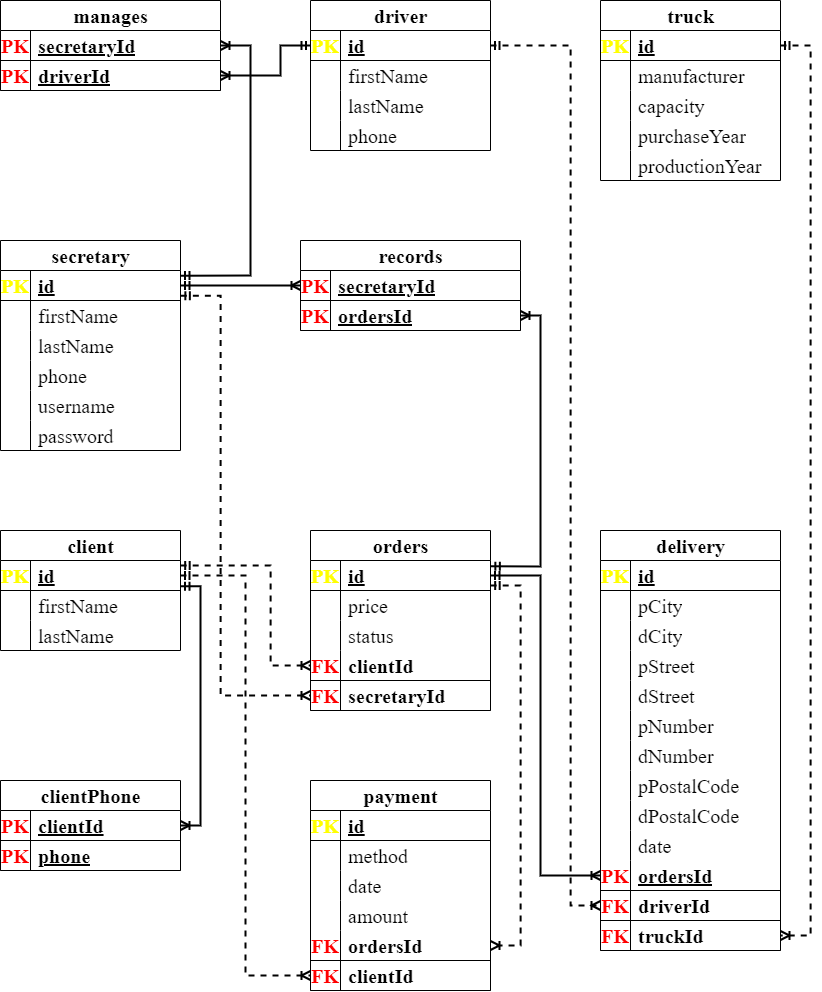
\includegraphics[width=0.6\textwidth]{images/RS.png}
  \captionsetup{labelfont=bf}
  \caption{Σχεσιακό Διάγραμμα}
\end{figure}

\newpage
\section{Ερωτήματα \foreignlanguage{english}{MySQL}}

\selectlanguage{English}
\begin{lstlisting}
---------- DATA ANALYSIS ----------

-- 1.) List the following details of each employee: 
------ employee number, last name, first name, sex, and salary.

SELECT concat(client.firstName, ' ', client.lastName) 
AS 'Client Name', orders.id AS 'Expected Orders'
FROM client, orders
WHERE orders.clientId = client.id 
		AND orders.status = 'Received';

SELECT concat(client.firstName, ' ', client.lastName) 
AS 'Client Name', payment.method
FROM client, payment
ORDER BY payment.method DESC;

SELECT * 
FROM client 
	JOIN payment ON client.id = payment.clientId;
    
SELECT concat(client.firstName, ' ', client.lastName) 
AS 'Client Name', payment.method, payment.amount, payment.date
FROM client
JOIN payment ON client.id = payment.clientId
WHERE payment.date BETWEEN '2023-05-05' AND '2023-09-09' 
ORDER BY DATE;

SELECT orders.id AS 'Orders'
FROM orders
WHERE status = 'Received'
UNION
SELECT delivery.id AS 'Deliveries'
FROM delivery
WHERE dCity = 'Xanthi';
\end{lstlisting}
\selectlanguage{greek}

%---------------------------------------------------------------------------------------------------------------
\newpage
\renewcommand{\chaptername}{Μέρος}
\chapter[Μέρος 3: Τελική Υλοποιήση Βάσης Δεδομένων]{Τελική Υλοποίηση Βάσης Δεδομένων}
\section{Άσκηση}
Καθολική Σχέση: R = {\foreignlanguage{english}{A, B, C, D, E, F, G, H, I, J}} 
\hfill \break
Σύνολο Συναρτησιακών Εξαρτήσεων: {\foreignlanguage{english}{$\{\{A\} \rightarrow \{J\}, \{E, A\} \rightarrow \{F\}, \{I\} \rightarrow \{G, D\}, \{E\} \rightarrow \{I, H\}, \{J\} \rightarrow \{C, B\}\}$ }}
\hfill \break
1. 



\begin{figure}[h]
  \centering
      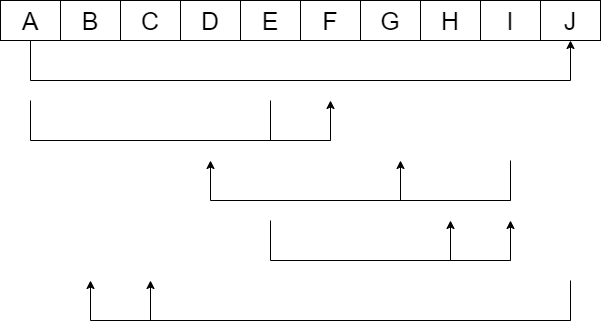
\includegraphics[width=0.8\textwidth]{images/diagram1.png}
  \captionsetup{labelfont=bf}
\end{figure}
\noindentΕφαρμόζουμε το θεώρημα που λέει ότι η κλειστότητα του κλειστού καθορίζει όλα τα γνωρίσματα. Τα \foreignlanguage{english}{B, C, D, F, G, H, I} και \foreignlanguage{english}{J} απορρίπτονται γιατί εξαρτώνται από κάποιο άλλο γνώρισμα και επομένως αντί για αυτά μπορούμε να χρησιμοποιήσουμε το γνώρισμα από το οποίο εξαρτώνται.
Τελικά προκύπτει ότι το κλειδί της R θα είναι το: \foreignlanguage{english}{$\{A, E\}$}$^+$.
\hfill \break
2. Να σπάσετε την \foreignlanguage{english}{R} σε σχέσεις που να βρίσκονται σε \foreignlanguage{english}{2NF}
\begin{figure}[h]
  \centering
      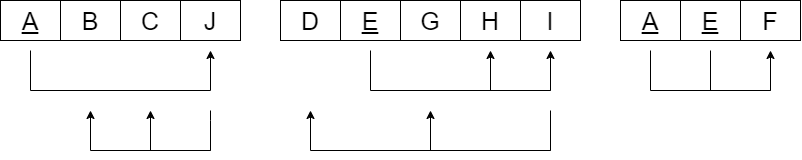
\includegraphics[width=0.8\textwidth]{images/diagram2.png}
  \captionsetup{labelfont=bf}
\end{figure}
\hfill \break
3. στη συνέχεια σε \foreignlanguage{english}{3NF}.
\hfill \break

\begin{figure}[h]
  \centering
      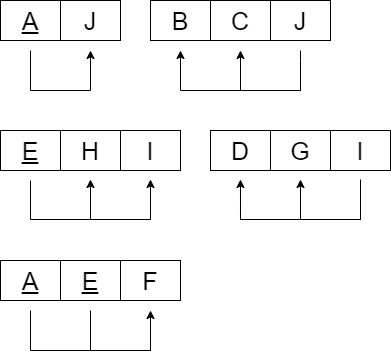
\includegraphics[width=0.6\textwidth]{images/diagram3.png}
  \captionsetup{labelfont=bf}
\end{figure}

\section{Κανονικοποίηση}
Οι δύο μεγαλύτεροι σε αριθμό γνωρισμάτων πίνακες της βάσης είναι \foreignlanguage{english}{SECRETARY} και \foreignlanguage{english}{DELIVERY}. Το σχήμα υποδεικνύει ότι τα κλειδιά που επιλέξαμε συμπίπτουν με αυτά που προκύπτουν από τις Σ.Ε. Οι πίνακες είναι σε \foreignlanguage{english}{2NF} και \foreignlanguage{english}{3NF} καθώς κάθε χαρακτηριστικό τους που δεν είναι κλειδί είναι συναρτησιακά εξαρτώμενο από το πρωτεύον κλειδί.
\begin{figure}[h]
  \centering
      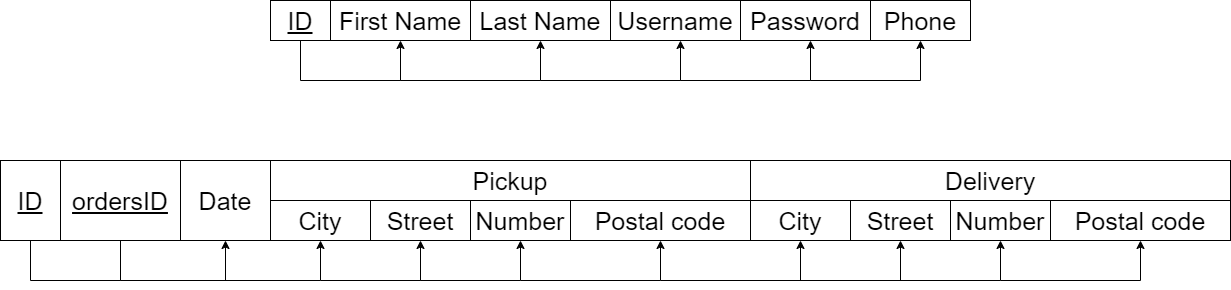
\includegraphics[width=1\textwidth]{images/diagram4.png}
  \captionsetup{labelfont=bf}
\end{figure}

\section{Ερωτήματα \foreignlanguage{english}{MySQL}}
\selectlanguage{English}
\begin{lstlisting}
----------# Queries 2----------
USE omada;

-- Both use JOIN with different reuslts --
-- #1 Total number of orders that have delivery
SELECT (SELECT COUNT(*) FROM orders INNER JOIN delivery 
    ON delivery.ordersID = orders.id) AS "Total Number Rows",
orders.id AS "Order ID", delivery.id AS "Delivery ID",
status AS Status, price AS Price, 
concat(dCity, ", ", dStreet, ", ", dNumber, ", ", dPostalCode) 
AS "Delivery Destination",
concat(pCity, ", ", pStreet, ", ", pNumber, ", ", pPostalCode) 
AS "Pick-Up Destination"
FROM orders
	INNER JOIN delivery ON delivery.ordersID = orders.id
ORDER BY CAST(orders.id AS SIGNED) ASC, date DESC, 
pCity ASC, dCity ASC;

-- #1 Total number of orders with and without delivery
SELECT (SELECT COUNT(*) FROM orders LEFT JOIN delivery 
ON delivery.ordersID = orders.id) AS "Total Number Rows",
orders.id AS "Order ID", delivery.id AS "Delivery ID", 
status AS Status, price AS Price, 
concat(dCity, ", ", dStreet, ", ", dNumber, ", ", dPostalCode) 
AS "Delivery Destination",
concat(pCity, ", ", pStreet, ", ", pNumber, ", ", pPostalCode) 
AS "Pick-Up Destination"
FROM orders
	LEFT JOIN delivery ON delivery.ordersID = orders.id;
    
-- #2 Average price of orders
SELECT avg(price) AS "Average Price"
FROM orders;

-- #3 Most recent delivery date 
SELECT MAX(date) AS "Average date"
FROM delivery;

-- #4 Group by method in payment entity
SELECT method AS Method, count(*) AS "Total Payments"
FROM payment
GROUP BY method
ORDER BY method ASC, count(*) DESC;

-- #5 Group by status in orders entity and using having command
SELECT  status, count(*) AS "Total Orders"
FROM orders
GROUP BY status
HAVING avg(price) > 300 AND status ="Received";
\end{lstlisting}


\selectlanguage{greek}

\section{Ευρετήρια}
Η δημιουργία ευρετηρίου για τα ονόματα της/του γραμματέα, της/του πελάτη και της/του οδηγού πιθανόν να είναι χρήσιμα για γρήγορη και αποτελεσματική αναζήτηση σε κάποια διεπαφή.
\hfill \break
Η δημιουργία ευρετηρίου για τις διευθύνσεις παραλαβής και παράδοσης μπορεί να διευκολύνει το προσωπικό της εταιρείας, όπως οι οδηγοί και οι γραμματείς, στον εντοπισμό και τη διαχείριση των παραδόσεων.

\selectlanguage{English}
\begin{lstlisting}
---------- CREATE INDEXES ----------
USE omada8;

---------- #1 create secretary full name index ----------
CREATE INDEX secretary_fullName_idk 
ON secretary(firstName, lastName);

---------- #2 create driver full name index ----------
CREATE INDEX driver_fullName_idk ON driver(firstName, lastName);

---------- #3 create client full name index ----------
CREATE INDEX client_fullName_idk ON client(firstName, lastName);

---------- #4 create delivery address index ----------
CREATE INDEX delivery_dAddress_idk 
ON delivery(dCity, dStreet, dNumber);

---------- #5 create pick-up address index ----------
CREATE INDEX delivery_pAddress_idk 
ON delivery(pCity, pStreet, pNumber);
\end{lstlisting}
\selectlanguage{greek}

\section{Όψεις}
Η πρώτη όψη δημιουργεί έναν εικονικό πίνακα που εμφανίζει τον αριθμό παραγγελίας, τον αριθμό παράδοσης, το όνομα του πελάτη, την διεύθυνση παραλαβής, την διεύθυνση παράδοσης, τον οδηγό που θα πραγματοποιήσει την παράδοση καθώς και τον αριθμό πινακίδας του εκάστοτε φορτηγού και ταξινομείτε με βάση τον αριθμό παραγγελίας. Θα μπορούσε να χρησιμοποιηθεί στην σελίδα της διεπαφής για να εμφανίσει τις σημαντικότερες πληροφορίες της παραγγελίας.
\hfill \break
Η δεύτερη όψη δημιουργεί έναν εικονικό πίνακα που εμφανίζει τον αριθμό παράδοσης και την ημερομηνία αποστολής που παραδόθηκαν τον τελευταίο χρόνο ταξινομημένα με βάση την ημερομηνία σε φθίνουσα σειρά. Θα μπορούσε να χρησιμοποιηθεί σε κάποια σελίδα της διεπαφής για να εμφανίσει τις πρόσφατες παραδόσεις.
\hfill \break


\selectlanguage{english}
\begin{lstlisting}
----------# Views ----------
USE omada8;

-- #1 create orders table with order by order id
CREATE OR REPLACE VIEW orders_table_view AS
SELECT orders.id AS "Order ID", 
delivery.id AS "Delivery ID", 
concat(client.firstName, ' ', client.lastName) AS "Client Name",
concat(pCity, ", ", pStreet, ", ", pNumber) AS "Pick-Up Dest",
concat(dCity, ", ", dStreet, ", ", dNumber) AS "Delivery Dest",
concat(driver.firstName, ' ', driver.lastName)
AS "Driver Full Name", truck.id AS "Truck ID"
FROM delivery
	INNER JOIN orders ON delivery.ordersId = orders.id
	INNER JOIN driver ON delivery.driverId = driver.id
	INNER JOIN truck ON delivery.truckID = truck.id
	INNER JOIN client ON orders.clientID = client.id
ORDER BY  CAST(orders.id AS SIGNED) ASC;

-- To show the results of the view 
SELECT * FROM orders_table_view;

-----------------------------------------------------------------

-- #2 create recent deliveries table order by date 
CREATE or REPLACE VIEW recent_deliveries_table_view AS
SELECT delivery.id AS 'Recent Deliveries', date
FROM delivery
WHERE date BETWEEN NOW() - INTERVAL 12 MONTH AND NOW()
ORDER BY delivery.date DESC;

-- To show the results of the view
SELECT * FROM recent_deliveries_table_view;
\end{lstlisting}
\selectlanguage{greek}

\section{Αποθηκευμένη Διαδικασία}
Η συγκεκριμένη αποθηκευμένη διαδικασία ανανεώνει την κατάσταση προϋπάρχουσας παραγγελίας.
\hfill \break
\selectlanguage{english}
\begin{lstlisting}
---------- Procedure ----------
USE omada8;

-- Task: Create a procedure to update existing order status 
-- in the orders table
DELIMITER !!
DROP PROCEDURE IF EXISTS UpdateOrderStatus;
CREATE PROCEDURE UpdateOrderStatus 
(IN orderIdParam VARCHAR(10), 
IN orderStatusParam enum('Received', 'Done', 'Cancel'))
BEGIN
    SET @orderID := (SELECT id 
                    FROM orders 
                    WHERE orders.id = orderIdParam);
    IF @orderID THEN
	    UPDATE orders SET status = orderStatusParam 
            WHERE id = orderIdParam;
            SELECT concat("Order ", orderIdParam,' is updated.')    
            AS Confirmation;
    ELSE 
	    SELECT 
            CONCAT("There is no order with id ", orderIdParam) 
            AS "Confirmation";
    END IF;
END !!
DELIMITER ;

-- To show the results of the procedure
CALL UpdateOrderStatus(11, "Done");

-- To verify tables are accurate after procedure
SELECT status FROM orders WHERE id = 11;
\end{lstlisting}

\selectlanguage{greek}

\section{Αποθηκευμένη Συνάρτηση}
Η συγκεκριμένη αποθηκευμένη συνάρτηση καταμετρά τον συνολικό αριθμό των παραδόσεων που έχει πραγματοποιήσει ένας οδηγός.
\hfill \break
\selectlanguage{english}
\begin{lstlisting}
---------- Procedure ----------
USE omada8;

-- Task: Create a function to retrieve the total number of 
-- deliveries for a specific driver
DELIMITER !
DROP FUNCTION IF EXISTS numberOfDeliveries;
CREATE FUNCTION numberOfDeliveries(driverLastName VARCHAR(30))
RETURNS INT
DETERMINISTIC
BEGIN
    DECLARE deliveryCount INT;

    SELECT COUNT(*)
    INTO deliveryCount
    FROM delivery
    INNER JOIN driver ON delivery.driverId = driver.id
    WHERE driverLastName = driver.lastName;

    RETURN deliveryCount;
END!
DELIMITER ;

-- To show the results of the procedure
SELECT numberOfDeliveries("Aggelidis") 
AS "The Total Number of Deliveries";
\end{lstlisting}
\selectlanguage{greek}

\section{Συνναλαγή}
\selectlanguage{english}
\begin{lstlisting}
---------- Transaction ----------

DROP PROCEDURE IF EXISTS test;

DELIMITER $$
CREATE PROCEDURE test() 
BEGIN
	DECLARE err TINYINT DEFAULT 0; 
	DECLARE CONTINUE HANDLER FOR SQLEXCEPTION SET err = 1;
    
	START TRANSACTION;
    
	INSERT INTO orders
		(id, price, status, secretaryID, clientID)
	VALUES
		(41, 300, 'Received', 6, 7);

	SAVEPOINT point1; 

	INSERT INTO delivery
	(id, pCity, pStreet, pNumber, pPostalCode, dCity, 
        dStreet, dNumber, dPostalCode, date, ordersID, 
        driverID, truckID)
	VALUES
	(20,'Komotini', 'Agios Dimitriou Street', 28, 69100, 
	'Alexandroupoli', 'Old Patras Street', 75, 69131, 
        '2023-06-21', 41, 1,'ZFK-5678');
    
	IF err = 1 THEN
		ROLLBACK TO SAVEPOINT point1;
		SELECT 'An error occurred' AS message;
	ELSE
		COMMIT;
		SELECT 'OK' AS message;
	END IF; 
    
END$$
DELIMITER ;

CALL test(); 

------------------------------------------------------------------
#verify tables are accurate
SELECT * FROM delivery WHERE id=20;

#verify tables are accurate
SELECT * FROM orders WHERE id=41;
\end{lstlisting}
\selectlanguage{greek}

\section{Σκανδάλη}
H δημιουργία αυτού του \selectlanguage{English}{trigger} ανανεώνει τo κόστος(\foreignlanguage{english}{amount}) της πληρωμής όταν πραγματοποιείται εισαγωγή της παραγγελίας και πιο συγκεκριμένα η τιμή(\foreignlanguage{english}{price}). Πρακτικά, αυτό σημαίνει ότι ο πελάτης καταχωρεί ένα πoσό προκαταβολής, το οποίο προστίθεται στο συνολικό κόστος της παραγγελίας.
\hfill \break
\selectlanguage{English}
\begin{lstlisting}
---------- Trigger ----------
USE omada8;

DELIMITER //
CREATE TRIGGER updateOrderPrice
AFTER INSERT ON payment
FOR EACH ROW
BEGIN
    UPDATE orders
    SET price = price + NEW.amount
    WHERE id = NEW.orderId;
END//
DELIMITER ;

---------- #verify tables are accurate ----------
INSERT INTO orders (id, secretaryID, clientID)
VALUES (18, 9, 4);

INSERT INTO payment (id, amount, date, clientID, orderID)
VALUES (18, 50.00, '2023-01-12', 2, 18);

SELECT * FROM orders WHERE id = 18;
\end{lstlisting}
\selectlanguage{greek}

%---------------------------------------------------------------------------------------------------------------
\titleformat{\chapter}[display]{\normalfont\huge\bfseries}{Κώδικας}{20pt}{\Huge}
\begin{appendices}
\chapter[Κώδικας: Τελική Υλοποιήση]{Τελική Υλοποίηση}

\pagestyle{mystyle}
\section*{Δημιουργία Βάσης Δεδομένων}
\addcontentsline{toc}{section}{Δημιουργία Βάσης Δεδομένων}
\selectlanguage{English}
\begin{lstlisting}
---------- SQL DATABASE ---------- Omada8

---------- CREATE DATABASE ----------

CREATE DATABASE omada8
	CHARSET 'utf8mb4' COLLATE 'utf8mb4_unicode_ci';

USE omada8;

---------- CREATE TABLES ----------

---------- #1 create secretary table [ENTITY] ----------
CREATE TABLE secretary(
    id VARCHAR(50) NOT NULL UNIQUE,
    firstName VARCHAR(50) NOT NULL,
    lastName VARCHAR(50) NOT NULL,
    phone BIGINT NULL DEFAULT NULL,
    username VARCHAR(50) NOT NULL,
    password VARCHAR(200) NOT NULL,
    
    CONSTRAINT pk_secretary PRIMARY KEY(id)
);

---------- #2 create driver table [ENTITY] ----------
CREATE TABLE driver(
    id VARCHAR(50) NOT NULL UNIQUE,
    firstName VARCHAR(50) NOT NULL, 
    lastName VARCHAR(50) NOT NULL,
    phone BIGINT DEFAULT NULL,
    
    CONSTRAINT pk_driver_id PRIMARY KEY(id)
);

---------- #3 create truck table [ENTITY] ----------
CREATE TABLE truck(
    id VARCHAR(50) NOT NULL UNIQUE,
    manufacturer VARCHAR(50) DEFAULT NULL,
    capacity  VARCHAR(10) DEFAULT NULL,
    purchaseYear YEAR DEFAULT NULL,
    productionYear YEAR DEFAULT NULL,
    
    CONSTRAINT pk_truck_id PRIMARY KEY(id)
);

---------- #4 create client table [ENTITY] ----------
CREATE TABLE client(
    id VARCHAR(50) NOT NULL UNIQUE,
    firstName VARCHAR(50) NOT NULL,
    lastName VARCHAR(50) NOT NULL,
    
    CONSTRAINT pk_client_id PRIMARY KEY(id)
);

---------- #5 create clientPhone table [RELATIONSHIP] ----------
CREATE TABLE clientphone(
    clientID VARCHAR(50) NOT NULL,
    phone BIGINT NOT NULL UNIQUE,
    
    CONSTRAINT pk_clientPhone PRIMARY KEY(clientID, phone),
    CONSTRAINT fk_clientPhone_clientId FOREIGN KEY(clientID) 
    REFERENCES client(id) ON DELETE CASCADE ON UPDATE CASCADE
);

---------- #6 create orders table [ENTITY] ----------
CREATE TABLE orders(
    id VARCHAR(50) NOT NULL UNIQUE,
    price DECIMAL(5, 2) NOT NULL DEFAULT 0.00,
    status ENUM('Received', 'Done', 'Cancel') NOT NULL 
    DEFAULT 'Received',
    
    secretaryID VARCHAR(50) NOT NULL,
    clientID VARCHAR(50) NOT NULL,
    
    CONSTRAINT pk_orders PRIMARY KEY(id),
    CONSTRAINT fk_orders_secretaryID FOREIGN KEY(secretaryID)  
    REFERENCES secretary(id) ON DELETE NO ACTION ON UPDATE 
    CASCADE,
    CONSTRAINT fk_orders_clientID FOREIGN KEY(clientID)  
    REFERENCES client(id) ON DELETE CASCADE ON UPDATE CASCADE
);


---------- #7 create payment table [ENTITY] ----------
CREATE TABLE payment(
    id VARCHAR(50) NOT NULL UNIQUE,
    amount DECIMAL(5, 2) NOT NULL,
    method ENUM('Cash', 'Card') NOT NULL DEFAULT 'Cash',
    date DATE NOT NULL,
    
    clientID VARCHAR(50) NOT NULL,
    orderID VARCHAR(50) NOT NULL UNIQUE,
     
    CONSTRAINT pk_payment PRIMARY KEY(id),
    CONSTRAINT fk_payment_clientID FOREIGN KEY(clientID) 
    REFERENCES client(id) ON DELETE CASCADE ON UPDATE CASCADE, 
    CONSTRAINT fk_payment_orderID FOREIGN KEY(orderID) 
    REFERENCES orders(id) ON DELETE CASCADE ON UPDATE CASCADE
);

---------- #8 create delivery table [ENTITY] ----------
CREATE TABLE delivery(
    id VARCHAR(50) NOT NULL UNIQUE,
    date DATE NOT NULL,
    pCity VARCHAR(50) NOT NULL,
    pStreet VARCHAR(50) NOT NULL,
    pNumber BIGINT NOT NULL,
    pPostalCode BIGINT NULL DEFAULT NULL,
    dCity VARCHAR(50) NOT NULL,
    dStreet VARCHAR(50) NOT NULL,
    dNumber BIGINT NOT NULL,
    dPostalCode BIGINT NULL DEFAULT NULL,

    ordersID VARCHAR(50) NOT NULL UNIQUE,
    driverID VARCHAR(50) NOT NULL,
    truckID VARCHAR(50) NOT NULL,
    
    CONSTRAINT pk_delivery PRIMARY KEY(id, ordersID),
    CONSTRAINT fk_delivery_ordersID FOREIGN KEY(ordersID) 
    REFERENCES orders(id) ON DELETE CASCADE ON UPDATE CASCADE,
    CONSTRAINT fk_delivery_driverID FOREIGN KEY(driverID) 
    REFERENCES driver(id) ON DELETE NO ACTION ON UPDATE CASCADE,
    CONSTRAINT fk_delivery_truckID FOREIGN KEY(truckID) 
    REFERENCES truck(id) ON DELETE NO ACTION ON UPDATE CASCADE
);

---------- #9 create manages table [RELATIONSHIP] ----------
CREATE TABLE manages(
    secretaryID VARCHAR(50) NOT NULL,
    driverID VARCHAR(50) NOT NULL,
    
    CONSTRAINT pk_manages PRIMARY KEY (secretaryID, driverID),
    CONSTRAINT fk_manages_secretaryId FOREIGN KEY(secretaryID) 
    REFERENCES secretary(id) ON DELETE NO ACTION ON UPDATE 
    CASCADE,
    CONSTRAINT fk_manages_driverId FOREIGN KEY(driverID) 
    REFERENCES driver(id) ON DELETE NO ACTION ON UPDATE CASCADE
);

---------- #10 create records table [RELATIONSHIP] ----------
CREATE TABLE records(
    secretaryID VARCHAR(50) NOT NULL,
    ordersID VARCHAR(50) NOT NULL,
    
    CONSTRAINT pk_records PRIMARY KEY (secretaryID, ordersID),
    CONSTRAINT fk_records_secretary FOREIGN KEY(secretaryID) 
    REFERENCES secretary(id) ON DELETE NO ACTION ON UPDATE 
    CASCADE,
    CONSTRAINT fk_records_ordersId FOREIGN KEY(ordersID) 
    REFERENCES orders(id) ON DELETE NO ACTION ON UPDATE CASCADE
);
\end{lstlisting}
\selectlanguage{greek}

\section*{Εισαγωγή Δεδομένων}
\addcontentsline{toc}{section}{Εισαγωγή Δείγματος Δεδομένων}
\selectlanguage{English}
\begin{lstlisting}
---------- INSERT MOCK DATA IN DATABASE ----------
USE omada8;

---------- #1 insert into secretary values ----------
INSERT INTO secretary (id, firstName, lastName, phone, 
username, password)
VALUES 
(1, 'Vasiliki', 'Miliou', 6950236484, 
'Penelope12', 'hgjhdghj'),
(2, 'Eirini', 'Fyssa', 6978543242, 
'NICK23', 'hewurhw' ),
(3, 'Panagiota', 'Papadopoulou', 6945426754, 
'CHASEKLOM', 'JIIEJhiuh'),
(4, 'Nefeli', 'Papadaki',6932401905, 
'12JENNIFER', 'bhuhdw'),
(5, 'Thanasis', 'Athanasiou', 6924164371, 
'J1OHthhr2NY', 'gwd2328'),
(6, 'Kostas', 'Dimitriou', 6947548910, 
'BETTEsc', '121ewdewFHHF2'),
(7, 'Giannis', 'Kontou', 6995847463, 
'MOSasxTEL', 'BCHDxsbsb2335'),
(8, 'Andreas', 'Panagiotou', 6954874263, 
'MATTHss12EW','123sajdh26'),
(9, 'Eleni', 'Tsironi', 6926154487, 
'JOEdwe','cdjc216emkm'),
(10, 'Philippos', 'Michailidis', 6978514263, 
'CHRISgvrgve1TIAN','GABLEjcjje');

---------- #2 insert into driver values ----------
INSERT INTO driver(id, firstName, lastName, phone)
VALUES
(1, 'Pyrrhos', 'Aggelidis','6971234567'),
(2, 'Epameinondas', 'Zafeiropoulos','6949274527'),
(3, 'Kassandra', 'Kyriakidi','6970013686'),
(4, 'Katerina', 'Dimitriou','6980536831'),
(5, 'Giannis', 'Karabatos','6949435810'),
(6, 'Petros', 'Kontos','6975542021'),
(7, 'Petros', 'Kontos','6975542021');

---------- #3 insert into truck values ----------
INSERT INTO truck(id, manufacturer, capacity, 
productionYear, purchaseYear)
VALUES
('ZFK-5678', 'Mercedes', '10 tons', '1999', '2009'),
('YKD-8899', 'Scania', '8 tons', '2008', '2010'),
('VRI-8753', 'Scania', '10 tons', '1999', '2010'),
('VRI-7753', 'Scania', '10 tons', '1999', '2010'),
('KOR-9981', 'Volvo', '10 tons', '1998', '2013'),
('KOR-9991', 'Volvo', '10 tons', '1998', '2013'),
('PLO-2266', 'Scania', '12 tons', '2001', '2015'),
('KEO-7185', 'Volvo', '8 tons', '2005', '2012');

---------- #4 insert into client values ----------
INSERT INTO client(id, firstName, lastName)
VALUES
(1, 'Giorgos', 'Kontogiannis'),
(2, 'Eleni', 'Markopoulou'),
(3, 'Nikos', 'Dimitrakopoulos'),
(4, 'Anastasia', 'Georgiou'),
(5, 'Dimitris', 'Karabasis'),
(6, 'Aikaterini', 'Michailidou'),
(7, 'Pavlos', 'Katsoulis'),
(8, 'Sofia', 'Liberopoulou'),
(9, 'Kostas', 'Papanikolaou'),
(10, 'Maria', 'Panagiotou'),
(11, 'Maria', 'Panagiotou'),
(12, 'Maria', 'Panagiotou');

---------- #5 insert into client phones values ----------
INSERT INTO clientPhone(clientId, phone)
VALUES
(1, 6810203041),
(1, 6452013687),
(2, 6958525654),
(3, 6958524565),
(4, 6945452564),
(4, 6845210395),
(5, 6898653212),
(6, 6484858689),
(7, 6959842364),
(8, 6465615253),
(8, 6987452034),
(8, 6954203956),
(9, 6845124793),
(10, 6456751520);

---------- #6 insert into orders values ----------
INSERT INTO orders(id, price, status, secretaryID, clientID)
VALUES
(1, 200, 'Received', 1, 1),
(2, 450, 'Received', 1, 1),
(3, 200, 'Done', 2, 3),
(4, 300, 'Done', 3, 4),
(5, 350, 'Done', 4, 5),
(6, 400, 'Received', 5, 6),
(7, 300, 'Received', 6, 7),
(8, 250, 'Received', 7, 8),
(9, 200, 'Done', 8, 9),
(10, 500, 'Received', 9, 10),
(11, 200, 'Done', 9, 5),
(12, 350, 'Done', 10, 5);

---------- #7 insert into payment values ----------
INSERT INTO payment(id, amount, method, date, clientID, orderID)
VALUES
(1, '250','Cash', '2023-05-21', 1, 1),
(2, '250','Cash', '2019-05-21', 1, 3),
(3, '250','Cash', '2019-05-21', 2, 2), 
(4, '250','Cash', '2019-05-21', 3, 12),
(5,'350','Card', '2023-02-07', 3, 4),
(6, '350','Card', '2023-11-30', 4, 5),
(7, '200','Card', '2023-09-03', 5, 6),
(8, '300','Cash', '2023-12-19', 6, 7),
(10, '400','Cash', '2023-09-17', 8, 8),
(11, '400','Cash', '2023-09-17', 9, 10),
(12, '400','Cash', '2023-09-17', 8, 11);

---------- #8 insert into delivery values ----------
INSERT INTO delivery(id, pCity, pStreet, pNumber, pPostalCode, 
dCity, dStreet, dNumber, dPostalCode, 
date, ordersID, driverID, truckID)
VALUES
(1,'Komotini', 'Agios Dimitriou Street', 28, 69100, 
'Alexandroupoli', 'Old Patras Street', 75, 69131, 
'2023-06-21', 1, 1,'ZFK-5678'),
(2,'Thessaloniki', 'Egnatias Street', 56, 54625, 
'Patra', 'Agios Nikolaos Street', 120, 26444, 
'2023-04-12', 2, 1, 'YKD-8899'),
(3,'Larisa', 'Ethnikis Antistasis Street', 9, 41222, 
'Xanthi', 'Dimitrakopoulou Street', 8, 67100, 
'2023-02-28', 3, 2, 'ZFK-5678'),
(4, 'Thessaloniki', 'Egnatias Street', 56, 54625, 
'Patra', 'Agios Nikolaos Street', 120, 26444, 
'2023-04-12', 4, 2, 'YKD-8899'),
(5, 'Tripoli', 'Leonidou Street', 45, 22131, 
'Thessaloniki', 'Demokratias Street', 42, 54631, 
'2023-01-26', 5, 7, 'PLO-2266'),
(6, 'Kalamata', 'Papaflessa Street', 20, 24100, 
'Larisa', 'Achilleos Street', 52, 41335, 
'2023-06-16', 6, 7, 'KEO-7185'),
(7, 'Kastoria', 'Megalous Alexandrou Street', 5, 52100, 
'Kozani', 'Papanastasiou Street', 10, 50123, 
'2023-02-22', 7, 1, 'ZFK-5678'),
(8, 'Serres', 'Aristotelous Street', 6, 62122, 
'Arta', 'Ioanni Karydi Street', 28, 47100, 
'2023-03-14', 8, 2, 'ZFK-5678'),
(9, 'Corinth', 'Ismenis Street', 18, 20100, 
'Lamia', 'Mesologgiou Street', 23, 35122, 
'2023-04-19', 9, 3, 'ZFK-5678'),
(10, 'Argos', 'Kapodistriou Street', 12, 21200, 
'Nafplio', 'Ioanninon Street', 40, 21100, 
'2023-02-10', 10, 3, 'ZFK-5678'),
(11, 'Corinth', 'Ismenis Street', 18, 20100, 
'Lamia', 'Mesologgiou Street', 23, 35122, 
'2023-04-19', 11, 4, 'ZFK-5678'),
(12, 'Corinth', 'Ismenis Street', 18, 20100, 
'Lamia', 'Mesologgiou Street', 23, 35122, 
'2023-04-19', 12, 2, 'ZFK-5678');

---------- #9 insert into manages values ----------
INSERT INTO manages(secretaryId, driverId)
VALUES
(2, 4),
(2, 5),
(2, 2),
(3, 3),
(4, 4),
(1, 1),
(6, 3),
(5, 5),
(3, 1);

---------- #10 insert into records values ----------
INSERT INTO records(secretaryId, ordersId)
VALUES
(1, 1),
(1, 7),
(1, 4),
(2, 2),
(2, 1),
(2, 7),
(2, 9),
(3, 3),
(3, 7),
(4, 4),
(4, 2),
(5, 4),
(5, 6),
(5, 5),
(6, 5),
(6, 6),
(7, 7),
(8, 8),
(9, 9),
(9, 10);

COMMIT;

--------------------------------------------------
--------------------------------------------------

USE omada8;

---------- verify tables are accurate ----------
SELECT count(*) FROM secretary; 
SELECT * FROM secretary;

SELECT count(*) FROM driver;
SELECT * FROM driver;

SELECT count(*) FROM truck;
SELECT * FROM truck;

SELECT count(*) FROM client;
SELECT * FROM client;

SELECT count(*) FROM clientPhone;
SELECT * FROM clientPhone;

SELECT count(*) FROM orders;
SELECT * FROM orders;

SELECT count(*) FROM payment;
SELECT * FROM payment;

SELECT count(*) FROM delivery;
SELECT * FROM delivery;

SELECT count(*) FROM manages;
SELECT * FROM manages;

SELECT count(*) FROM records;
SELECT * FROM records;
\end{lstlisting}
\selectlanguage{greek}
\end{appendices}

%---------------------------------------------------------------------------------------------------------------
\nocite{elmasri2011fundamentals}

\bibliographystyle{abbrv}
\textlatin{\bibliography{references/bibl}}
\addcontentsline{toc}{chapter}{Βιβλιογραφία}

\end{document}
